\chapter{Electrical Systems}
Take a short look at the whole text before starting to write your part.
\section{Introduction}
% Electrical introduction content here

\subsection{(b) List of all discrete electrical subsystems.}
We are implementing the following subsystems: 
\begin{itemize}
    \item LV Battery
    \item HV Power Supply, including \begin{itemize}
        \item Battery Management System
        \item Insulation Monitoring Device
    \end{itemize}
    \item Traction Inverter
    \item Propulsion Motor    
    \item Sense and Control System
\end{itemize}

\subsection{(a) Brief overview with the main points of the HV and LV systems.}
Our electrical system provides the electrical power for the propulsion and control systems. We have a low voltage circuit nominally rated at 24V (for control systems) and a high voltage level circuit at 444V (for the traction system).
The low voltage circuit activates and controls the high voltage power supply through the Battery Management System and is hence designed for reliability. \\
The high voltage circuit is designed for safety, being potentially lethal, and power, in order to maximize the use of the motor. An OEM Insulation Monitoring Device checks for the (lack of) resistance between chassis and the HV power line in case of short circuits. \\
The traction inverter uses the electric power of
the high voltage battery to power the motor, 
converting DC power into AC phases. We use an 
OEM device that is used in automotive purposes. 
\\
\par The motor is a lightweight motor from Emrax. Even though it belongs to the traction system,
we will document it in the electrical section, 
as the development team of the originally
planned inhouse-built inverter took over the 
duty of the electrical part of the
motor system, too.
\par The Sense and Control System is not part of the EHW definition of the electrical systems. Since we have to provide a documentation nonetheless and the team designing the electrical subsystem also designed the Sense and Control system, we decided to include it as a part of the electrical subsystem documentation. It controls the brakes, the thermal pump, the telemetry line and the telemetry unit, as well as additional physical sensors. 

\par Our general design of this season is inspired by conventional modes of transportation,
as we have not had the capacity to start developing a levitation system by this season
Thus, we focussed on an electrical system that drives our friction-based motor with
excelling acceleration, which is a problem that railway systems frequently face.

\par In between design and production phase, we received a sponsorship of Leadrive,
a local startup for research on automotive power electronics.
Furthermore, the institute for electrical systems (ISEA) of our home university offered us assistance in the production of battery cells.
Therefore, our workload was eased, which turned out to be favorable
because of our lack of team members in the electrical field. This has been a crucial
constraint in the design and planning process of the electrical department
since the last season. Only shortly before submitting the ITD, we were able to make an estimation of
realistic goals for the new team.

\par This year, we would like to set the path for magnetic levitation in the future, relying on an active system
inside the vehicles. This was taken into consideration when designing the power dimensions,
keeping plenty of overhead for the future, which aligns with our goal of sustainability.
By having reusable modules, the design process of the upcoming years will be simplified.

\par We collaborate with the following institutions for support in the electrical department (including S\&C):
\begin{itemize}
    \item \textbf{Altium:} Sponsored Licenses of PCB design software
    \item \textbf{Festo:} Sponsored mechanical components and sensors for pneumatic systems.
    \item \textbf{Mouser Electronics:} Sponsored certain electronics.
    \item \textbf{Würth Elektronik:} Sponsored certain electronics.
    \item \textbf{Leadrive:} Sponsored traction inverter
    \item \textbf{Vector Informatik:} Sponsored CANoe Suite, including technical training for CAN networks.
    \item \textbf{Bender:} Sponsored Insulation Monitoring Device.
    \item \textbf{ISEA:} Assembling our battery pack.
\end{itemize}



\subsection{(c) Wiring diagram of the HV system.}
To Sourajit.

\section{LV Battery}
\subsection{Overview}
\graphicspath{ {./texfiles/electrical/eimc/} }
%Electrical overview content here
\subsubsection*{Main requirements and constraints that drive the design}
\par Our Low Voltage system drives all electrical and digital control systems of the Fermion, which 
is equivalent to all electronic systems but the inverter for propulsion. As stated previously,
reliability is crucial in this case. A failure of any component may lead to the shutdown of critical systems, such as the battery management system.
Furthermore, an overvoltage may potentially damage these systems, causing safety hazards. We had the option between building a LV battery pack from spare LiPo cells we ordered for the HV battery pack, and using automotive-grade ventilated lead-acid batteries.
After considering the safety problems of LiPo cells and the efforts of either building a second (smaller) LV BMS or taking the risk of having a singular point of failure by controlling both systems with the same BMS, powering the BMS with the cells it controls, we went for the approach with lead-acid batteries, that is widely used in automotive systems. It is regarded as more reliable and robust compared to the Lithium-Ion pendants that we use for the High Voltage System. \\
Furthermore, the safety risks of lead-acid batteries are much lower than those of LiPo cells, for example in the case of
crashes and overcharging/overdischarging.\\
\subsubsection*{Power requirements}
We consider the power consumption of all components in the low voltage power line for the power requirements:
\begin{itemize}
    \item \textbf{Solenoid Valves:} According to the data sheet, the valves use 2.25 Watts à 4 valves = 9 Watts. While switching, which takes 3.5 ms, they use 8.5 Watts.
    Assuming that we switch all four valves 20 times, we have an additional consumption of \(0.595 J\), which is almost negleglible. We will assume a power consumption of 10 Watts for tolerance.
    \item \textbf{Thermal Pump:} Given the water flow rate, we calculated a theoretical need of 34 Watts for the pump. As we do not have experimental data, we assume that 75 Watts are required at maximum.
    
    \item \textbf{Raspberry Pi 4:} One Raspberry Pi 4B consumes \(10 \, \text{Watts}\).
    \item \textbf{Raspberry Pico W:}
    \item One Raspberry Pico W does not consume more than \(1 \, \text{Watt}\). 

    \item \textbf{Microcontrollers (TIC2000 F280039C):}
    \begin{itemize}
        \item According to datasheet, one microcontroller uses \(3.3V * 0.11 A = 0.363 W \). The controller circuits will not exceed 5 Watts in total. 
    \end{itemize}

    \item \textbf{BMS (Orion BMS 2, 180 Cells):}
       Our BMS consumes up to 2 Watts, according to the datasheet.

    \item \textbf{Leadrive Inverter:} Using the nominal power ratings of 3 A at 24 V, we have a power consumption of 72 Watts. The producer informed us that the average consumption is significantly lower,
    which we confirmed after testing the inverter with no load, which uses approximately 25 Watts.
    \item \textbf{IMD}: Our IMD consumes up to 2 Watts, according to the datasheet.
    \item Network transceiver: We use the Rocket M2, which consumes up to 6 Watt of energy, according to the datasheet.
    \item Precharge relay and contactors: Our precharge relay uses \(0.32 W \), our main contactors use \(2 * 12V * 1A\) in total. We will calculate with 25W.
\end{itemize}

Now, summing up all the (excessively computated) power requirements, we have
\(10W + 50W + 10W + 1W + 5W + 2W + 72W + 2W + 6W + 25W = 183W \) , which is roughly 7.7 A at 24V. \\
Using the discharge chart of the data sheet of the LV Battery,
\begin{wrapfigure}{r}{0.25\textwidth}
    \centering
    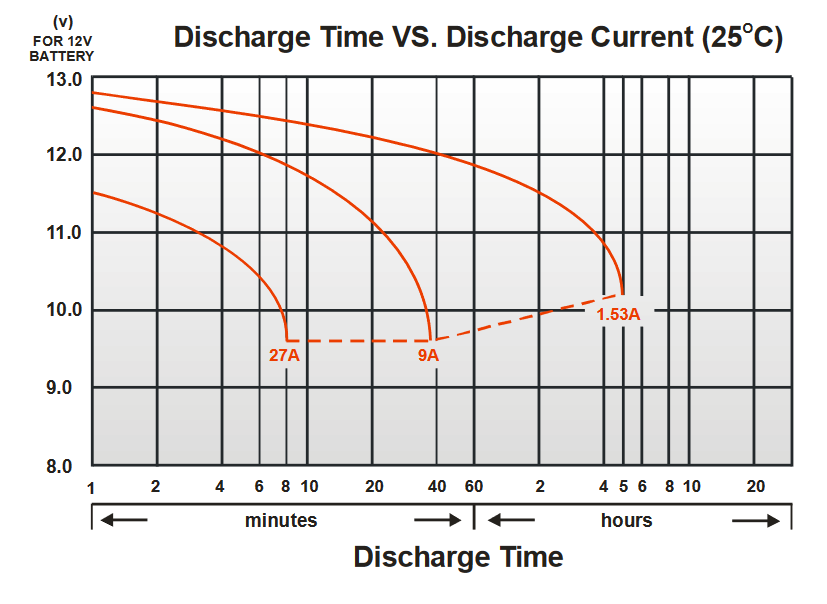
\includegraphics[width=0.25\textwidth]{texfiles/elec/eimg/LV_Battery_WP1236W}
    \caption{Discharge chart of LV battery cell}
\end{wrapfigure}
it is evident that even at full power (9A - including some headroom for losses), we can run our low voltage system for 20 minutes. During the competition, we can rule out that we will use that much power over the whole 20 minutes. 
Assuming that the pump is activated while the HV system is at work, and that this duration takes 2 minutes maximum (the actual run will be much less - max. 20 seconds), and we assume only a usage of 111 W for the rest of the time,
we can use the LV battery for well over 20 minutes. \\
In conclusion, the capacity of 9Ah is a trade-off between the mass and the available runtime of the system.
\subsection{Electrical and mechanical design process}
%Electrical and mechanical design process content here
\subsubsection{Schematic}
\begin{figure}[h]
    \centering
    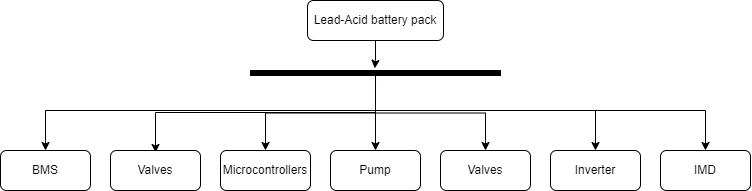
\includegraphics[width=0.75\textwidth]{texfiles/elec/eimg/LV_Diagram}
    \caption{Diagram of LV connections}
\end{figure}
\begin{figure}[h]
    \centering
    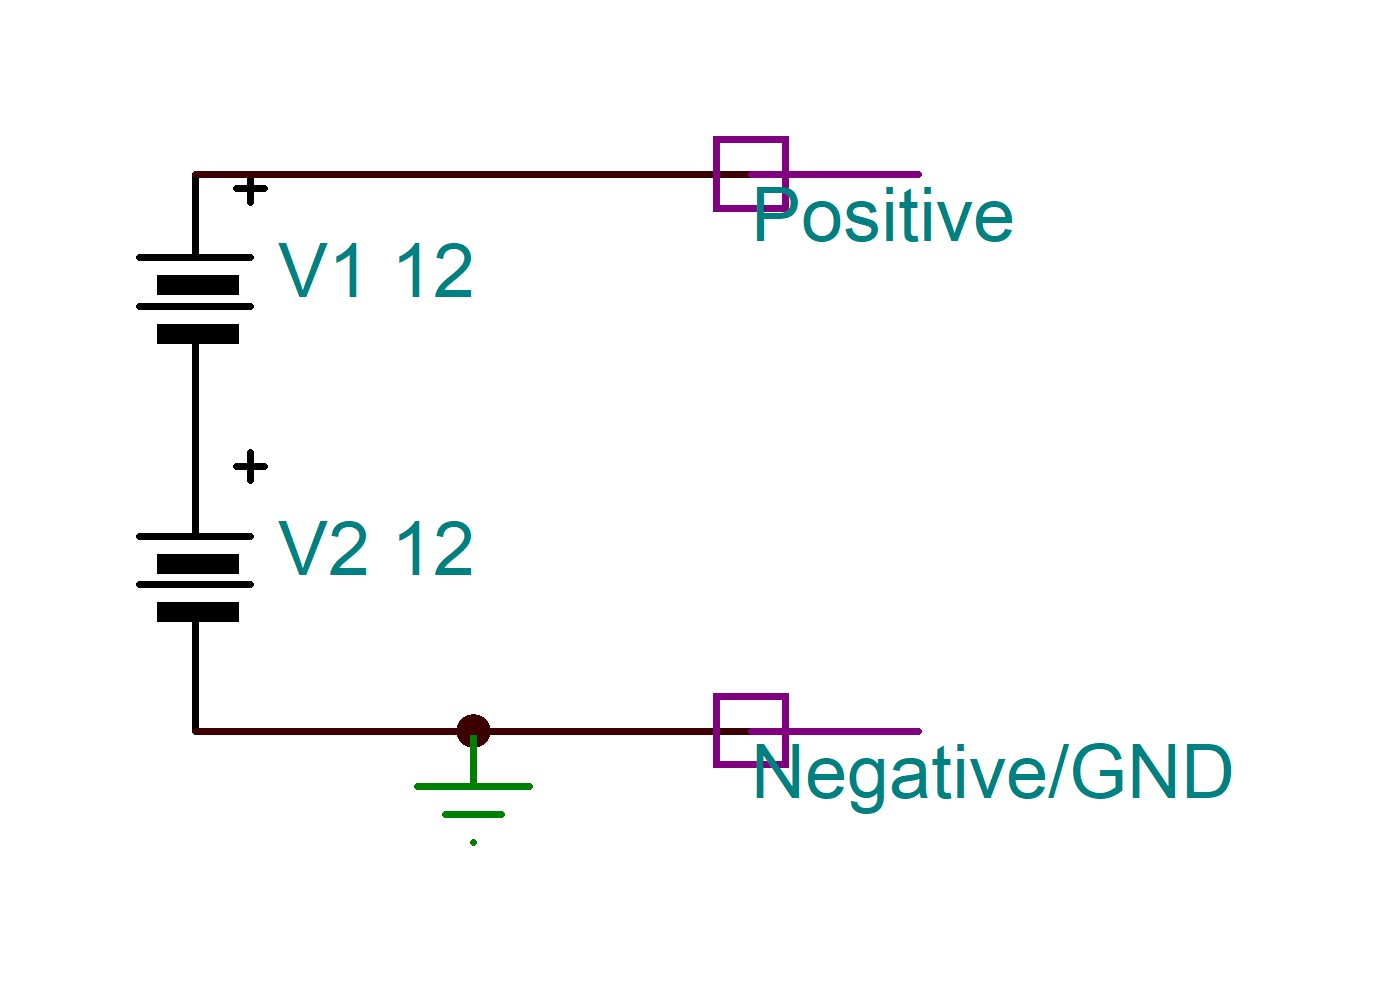
\includegraphics[width=0.5\textwidth]{texfiles/elec/eimg/LVCircuit}
    \caption{Schematic of LV battery cell}
\end{figure}
\subsubsection{(b) Present temperature simulations for vacuum conditions.}
We did a rough estimation based on the internal resistance of the
battery, which is around \(0.014 \Omega \) according to the datasheet. We will assume \(0.02 \Omega\). Using the equation of heat loss, we get \(P = I^2 * R = 8^2 * 0.02 * W = 1.28W\).\\
The ... Bohdan \\


For our heat simulations, we used the software of ANSYS. By vacuum conditions, we assumed the
lack of gas flow, which eliminates the cooling heat flow from winds. The simulation tool solves
the heat transfer equation \( \frac{\partial T}{\partial t} = \alpha \left( \frac{\partial^2 T}{\partial x^2} + \frac{\partial^2 T}{\partial y^2} + \frac{\partial^2 T}{\partial z^2} \right) \)
by discretizing through Finite-Element-Methods.

\subsection{Electrical system characteristics}
%Content of the electrical system characteristics here
\begin{table}[h]
    \centering
    \begin{adjustbox}{width=\textwidth,center}
    \begin{tabular}{|c|c|}
       \hline
       Battery Type & Lead-Acid(integrated)\\
       \hline
       Capacity[Ah] & 9 \\
       \hline
       Nominal Voltage[V] & 12 \\
       \hline
       Cell configuration & 2s \\
       \hline
       Max. discharge [A] & 10 \\
       \hline
       Weight per cell [Kg] & 2,7 \\
       \hline 
       Dimensions per cell (L x W x H)[mm] & 151 x 65 x 94 \\
       \hline 
    \end{tabular}
    \end{adjustbox}
    \label{Low Voltage Cell Specs}
    \caption{LV battery cell characteristics}
\end{table}    

\begin{table}[h]
    \centering
    \begin{adjustbox}{width=\textwidth,center}
    \begin{tabular}{|c|c|}
       \hline
       Battery Type & Lead-Acid(integrated)\\
       \hline
       Capacity[Ah] & 9 \\
       \hline
       Nominal Voltage[V] & 24 \\
       \hline
       Cell configuration & 2s \\
       \hline
       Max. discharge [A] & 10 \\
       \hline
       Weight [Kg] & 5.5 \\
       \hline 
       Dimensions (L x W x H)[mm] & 151 x 65 x 94 \\
       \hline 
    \end{tabular}
    \end{adjustbox}
    \label{Low Voltage Battery Specs}
    \caption{LV battery pack characteristics}
\end{table}    

\subsection{Interface with other system}
%Interface with other system content here n
All the electric subsystems are located within the pod. \\
It powers the entire sensing, control and telemetry system. 
The LV battery itself does not communicate. Its sensor data is processed by the thermal control board.
When the voltage drops below a certain threshold, the complete system shuts down.

\subsection{Final system description}
%Description of the system here
The two lead-acid batteries, chained in series, provide a nominal voltage of 24V (12V each). When fully charged, the voltage can increase up to 26 V. The lead acid batteries' voltage will drop while discharging. Hence, we monitor the voltage while using the LV battery system. Furthermore, we monitor the temperature through a NTC thermistor to prevent usage under overtemperature . \\
The 24 V power source gets transferred down to 12V (for the Thermal Pump) and 5V for the micro-controllers by buck converters, and drives the valves and several sensors at 24V simultaneously. \\
After reaching out to the EHW technical committee, we were able to clarify that a BMS, used by Lithium-Ion batteries, is not required for lead-acid batteries due to the inherently different chemical structure which makes over- and undercharging much less critical. \\
For charging, we are using a battery charger specified for 12V and 24V lead acid cells from Würth 0510955908. The charging of lead-acid batteries in series is unproblematic, given that we regularly test for drifts and manually balance the cells.\\

\subsection{Manufacturing process}
%Manufacturing process content here
As the cells come in hard-shell covers already, the manufacturing process is not very complicated. We will 3D-print a case from Polycarbonate material which permits flow of air and prevents short circuits physically.

\subsection{Testing}
%Testing content here
We will test whether the lead acid cells and the thermistors are accurate to their datasheet. This especially includes \begin{itemize}
    \item the capacity of the packs at 9A discharge (according to real scenario)
    \item the heat development while discharging
\end{itemize}
    %\subsection{FMEA}
%FMEA content here


\section{High Voltage Power Supply}
\subsection{Overview}
%Electrical overview content here
(a) Explain the main requirements and constraints that drive the design. \\


\subsection{Electrical and mechanical design process}
%Electrical and mechanical design process content here
\subsubsection{(a) Present Schematics or logic diagrams of the boards.}
\subsubsection{(b) Present temperature simulations for vacuum conditions.}
For our heat simulations, we used the software of ANSYS. By vacuum conditions, we assumed the
lack of gas flow, which eliminates the cooling heat flow from winds. The simulation tool solves
the heat transfer equation \( \frac{\partial T}{\partial t} = \alpha \left( \frac{\partial^2 T}{\partial x^2} + \frac{\partial^2 T}{\partial y^2} + \frac{\partial^2 T}{\partial z^2} \right) \)
by discretizing through Finite-Element-Methods.

\subsection{Description of subsystem control}
%Description of subsystem control content here
\subsubsection{(a) Briefly reference the control systems of the boards, which should be explained in the levitation or propulsion subsection respectively.}
We configure the BMS prior to the competition. \\


\subsection{Electrical system characteristics}
%Content of the electrical system characteristics here
   


\subsection{Interface with other system}
%Interface with other system content here n
(a) Briefly reference the communication protocols or control mechanisms of the boards, which should be explained in the respective Sense and Control subsection. \\
All the electric subsystems are located within the pod. \\

The phsyical connection matrix is as following:
\begin{table}
    \centering
    \begin{adjustbox}{width=\textwidth,center}
    \begin{tabular}{|c|c|c|c|c|c|c|}
    \hline
    From | To & \text{LV Battery} & \text{HV Battery} & \text{BMS} & \text{Traction Inverter} & \text{Motor} & \text{Cooling System} \\
    \hline
    \text{LV Battery} & - & - & Powers & \text{Powers control system} & - & \text{Powers pump and control system} \\
    \hline
    \text{HV Battery} & - & - & Connects to & \text{Provides power} & - & - \\
    \hline
    \text{BMS} & - & - & \text{Controls} & - & - & - \\
    \text{Traction Inverter} & - & - & - & - & \text{Propels} & X \\
    \hline
    \text{Motor} & - & - & - & - & - & - \\
    \hline
    \text{Cooling System} & - & - & - & \text{Cooling} & \text{Cooling} & \text{Cooling (implicitly)} \\
    \hline
    \end{tabular}
\end{adjustbox}
\caption{Physical connection matrix}
\label{Physical connection matrix Battery}
\end{table}

The data connection matrix is as following. All communication between boards are via CAN, if not specified otherwise:

\begin{table}
    \centering
    \begin{adjustbox}{width=\textwidth,center}
    \begin{tabular}{|l|c|c|c|c|c|c|c|c|}
    \hline
    From $\backslash$ To & LV Battery & HV Battery & BMS & Traction Inverter & Motor & Cooling System & Brakes Controller & Telemetry Unit  \\
    \hline
    LV Battery & - & - & - & - & - & - & - & - \\
    HV Battery  & - & - & Discharge rate, voltage level & - & - & - & - & - \\
    BMS & controls & controls & - & - & - & - & - & sends data \\
    Traction Inverter & - & - & - & - & - & - & - & sends data \\
    Motor & - & - & - & - & - & - & - & - \\
    Cooling System & - & - & - & - & - & - & - & sends data \\
    Brakes Controller & - & - & - & - & - & - & - & sends data \\
    Telemetry Unit & - & - & updates limits & sends commands & - & sends target rates & sends commands & - \\
    \hline
    \end{tabular}
    \end{adjustbox}
    \caption{Data connection matrix}
    \label{data-connectivity-matrix-battery}
\end{table}


\subsection{Final system description}
%Description of the system here
\subsubsection{Battery Cells}

High Voltage Network:

Our high voltage battery will make use of lithium-ion polymer technology. We use 120 pouch-format cells from Shenzhen GrePow Battery Co. Ltd rated at 45C maximum discharge that we plan to connect in series. 
The finished package (main battery pack) will be assembled by the team.
We are going to connect the 120 cells connected in series and that will have 1 parallel line. This will roughly have 504 Volt at max (using \(120 * 4.2V = 504 V \) ) 
which provides sufficient electricity to power the motor.
The battery pack will provide up to ~350 Amps of DC current available to the inverter. However, neither the inverter nor the motor is not rated for such high currents nominally. 
\newline
Therefore, the maximum output current of the HV Battery will be rated at 200 A maximum (peak) and 100 A continuous. 

We will stack 30 cells in series per pack and then stack 4 of them to get the full battery pack. No we won't.
\newline
\subsubsection{BMS}
Our battery management system 

The Orion BMS 2, connected to the HV battery, protects it and improves its life, efficiency. 
Operational Mechanics

The Orion BMS 2 facilitates real-time monitoring and management of each cell within the HV battery pack, 
which consists of 120 lithium-ion polymer cells arranged in a series configuration to achieve a nominal voltage of 504V. 
This arrangement necessitates precise control and monitoring to prevent overcharging, deep discharging, and to ensure balanced 
cell voltages, all of which are within the Orion BMS 2's capabilities.

1. **Cell Voltage Monitoring and Balancing:** The BMS continuously monitors the voltage of each cell, ensuring 
that all cells operate within their safe voltage range. Cell balancing is performed to equalize the charge across all cells,
thereby enhancing the battery pack's overall efficiency and lifespan.

2. **Temperature Monitoring:** 
Given the high energy density of the HV battery pack, 
thermal management is paramount. The Orion BMS 2 monitors the temperature of individual cells 
and the battery pack as a whole, activating cooling measures when necessary and preventing operation 
under extreme temperatures that could damage the battery or compromise safety.
The Orion BMS 2 itself tracks the temperature of 8 individual cells. 28 other cells are measured by the Thermal Controller.

3. **State of Charge (SoC) and State of Health (SoH) Estimation:** 
SoC and SoH estimations are important for optimal battery utilization and health maintenance. 
The Orion BMS 2 employs advanced algorithms to provide these estimates, 
ensuring that the battery's capacity is used efficiently.


The integration of the Orion BMS 2 encompasses several safety mechanisms designed to protect the battery pack, the hyperloop pod, and its occupants:

1. **Overcurrent and Short Circuit Protection:** By monitoring the current flowing in and out of the battery pack, the Orion BMS 2 can detect overcurrent conditions and short circuits, initiating immediate shutdown procedures to prevent damage and ensure safety.

2. **High and Low Voltage Protection:** The BMS prevents the battery from exceeding its maximum voltage during charging and dropping below its minimum voltage during discharge, thereby avoiding scenarios that could lead to reduced battery life or safety hazards.

3. **Thermal Runaway Prevention:** Through its temperature monitoring capabilities, the Orion BMS 2 can detect the onset of thermal runaway—a dangerous condition where one cell's failure can lead to a cascading failure of adjacent cells—and take corrective actions to isolate the problem and mitigate potential damage.

Efficiency Enhancements

By optimizing the operational parameters of the HV battery pack, the Orion BMS 2 contributes significantly to the efficiency and performance of the hyperloop prototype:

1. **Energy Optimization:** By ensuring that all cells are balanced and operate within their optimal voltage and temperature ranges, the BMS maximizes the energy extracted from the battery pack, contributing to the hyperloop's range and speed capabilities.

2. **Lifecycle Extension:** Through diligent monitoring and management, the Orion BMS 2 extends the useful life of the HV battery pack, reducing the environmental impact and operational costs associated with battery replacement.

3. **Predictive Maintenance:** By providing detailed data on the SoC and SoH, the Orion BMS 2 enables predictive maintenance, allowing for timely interventions that prevent unscheduled downtimes and extend the battery's lifespan.

Conclusion

The integration of the Orion BMS 2 with the HV battery pack in our hyperloop prototype represents a critical step towards ensuring the system's safety, efficiency, and reliability. Through its comprehensive monitoring and management capabilities, the Orion BMS 2 ensures that the HV battery pack operates within its optimal parameters, significantly contributing to the prototype's overall performance and safety profile. As we progress towards the final stages of the FDD, the detailed exploration of the Orion BMS 2's functionalities underscores our commitment to leveraging advanced technologies for the enhancement of hyperloop transportation systems.
\subsubsection{Insulation Monitoring Device}
The Insulation Monitoring Device that is mandatory for EHW participants, as well as Formula Students teams, is not built inhouse, after receiving the respective advice from the EHW technical jury. By reaching out to Bender, we received their device through their Formula Students policy. It is configured for ...


\subsection{Manufacturing process}
%Manufacturing process content here
Our PCB Design
\subsubsection{PCBs}
\par Prototyping: Prototype PCBs are fabricated in the FabLab associated with our university. The FabLab provides access to PCB manufacturing equipment and materials, enabling the rapid production of prototypes for initial testing and design validation.
    Once the PCBs are fabricated, they are assembled manually by our team members. Bigger PCBs are assembled in the facilities of the FabLab with the manual Pick and Place Machine and a reflow oven.
\par Production: We ordered our final PCBs from JLCPCB, a leading PCB manufacturing service. In addition to JLCPCB, we also collaborate with Würth Elektronik who produce 
PCBs in Germany, aligning with our goal of sustainability.
\subsubsection{Batteries}
The production of the low voltage battery pack is rather easy. We will use a 3d printer to print the casing
We produced the battery packs in cooperation with the ISEA (Institute for Power Electronics and Electrical Drives) at RWTH, whose experience helped us to assemble and design the parts
more efficienciently and more safely, as we had a considerable high voltage system.
The casing will consist of polycarbonate. Polycarbonate is a material that is
durable , lightweight, and impact resistant. The problems with
material degradation through UV emissions does not impact us substantially, as we
cover the battery pack inside the shell for most of the time. We will have safety measures preventing too much exposure to UV radiation.
Also, the degradation is mainly of cosmetic nature (https://link.springer.com/article/10.1007/s11668-020-01002-9) .

\subsection{Testing}
%Testing content here
We started testing software.

%\subsection{FMEA}
%FMEA content here


\section{Power Electronics}
\section{Power Electronics}

\subsection{Introduction}
We have a motor.
\subsubsection{FDD.9 Budget, Funding, and Manufacturing Methods}
 
\subsection{Technical Description and Constraints}
\subsubsection{FDD.11 Technical Specifications}

\subsubsection{FDD.17 Design Constraints}
 
\subsubsection{FDD.18 Performance Requirements}
 
\subsubsection{FDD.19 Integration with Other Systems}
 
\subsection{Objectives and Design Approach}
\subsubsection{FDD.12 Design Objectives}
 
\subsubsection{FDD.15 Innovative Aspects}
 
\subsubsection{FDD.16 Design Approach}
 
\subsection{Safety}
\subsubsection{FDD.13 Safety Considerations}
 
\subsubsection{FDD.14 Safety Testing and Compliance}
 
\subsection{Parts List (FDD.21)}
% Comprehensive list of all parts used in the braking system, including specifications and suppliers.

\begin{table}[h]
    \centering
    \caption{Parts List}
    \begin{tabular}{|p{0.7cm}|p{4cm}|p{4cm}|p{3cm}|p{0.7cm}|p{1cm}|p{1cm}|}
        \hline
        \textbf{Amount} & \textbf{Name} & \textbf{Company, (Serial Number)} & \textbf{Dimensions [mm x mm x mm]} & \textbf{Weight [kg]} & \textbf{Nominal Voltage} & \textbf{Expected max current} \\
        \hline
        1 & Power Inverter & Leadrive EV0019 & 300x300x150 & 9 & 800V & 200A \\
        \hline
        1 & Motor & Emrax 188AC & 200x200x200 & 15 & 120V & 50A \\
        \hline

    \end{tabular}
\end{table}


\newpage

\section{Sensing and Control}
\section{Sensing and Control}

\subsection{Introduction}
\subsubsection{FDD.9 Budget, Funding, and Manufacturing Methods}
 
\subsection{Technical Description and Constraints}
\subsubsection{FDD.11 Technical Specifications}
 
\subsubsection{FDD.17 Design Constraints}
 
\subsubsection{FDD.18 Performance Requirements}
 
\subsubsection{FDD.19 Integration with Other Systems}
 
\subsection{Objectives and Design Approach}
\subsubsection{FDD.12 Design Objectives}
 
\subsubsection{FDD.15 Innovative Aspects}
 
\subsubsection{FDD.16 Design Approach}
 
\subsection{Safety}
\subsubsection{FDD.13 Safety Considerations}
 
\subsubsection{FDD.14 Safety Testing and Compliance}
 
\subsection{Parts List (FDD.21)}
% Comprehensive list of all parts used in the braking system, including specifications and suppliers.

\newpage

\section{Additional considerations when writing the document for specific subsystems}
%Additional considerations when writing the document for specific subsystems content here
Sources:
\begin{itemize}
    \item https://link.springer.com/article/10.1007/s40789-022-00494-0 BMS System Reliability
    \item 
\end{itemize}


%%%%
\begin{comment}
\subsection{Overview}
%Electrical overview content here
(a) Explain the main requirements and constraints that drive the design. \\


\subsection{Electrical and mechanical design process}
%Electrical and mechanical design process content here
\subsubsection{(a) Present Schematics or logic diagrams of the boards.}
\subsubsection{(b) Present temperature simulations for vacuum conditions.}
For our heat simulations, we used the software of ANSYS. By vacuum conditions, we assumed the
lack of gas flow, which eliminates the cooling heat flow from winds. The simulation tool solves
the heat transfer equation \( \frac{\partial T}{\partial t} = \alpha \left( \frac{\partial^2 T}{\partial x^2} + \frac{\partial^2 T}{\partial y^2} + \frac{\partial^2 T}{\partial z^2} \right) \)
by discretizing through Finite-Element-Methods.

\subsection{Description of subsystem control}
%Description of subsystem control content here
\subsubsection{(a) Briefly reference the control systems of the boards, which should be explained in the levitation or propulsion subsection respectively.}
We configure the BMS prior to the competition. \\


\subsection{Electrical system characteristics}
%Content of the electrical system characteristics here
   


\subsection{Interface with other system}
%Interface with other system content here n
(a) Briefly reference the communication protocols or control mechanisms of the boards, which should be explained in the respective Sense and Control subsection. \\
All the electric subsystems are located within the pod. \\

The phsyical connection matrix is as following:
\begin{table}
    \centering
    \begin{adjustbox}{width=\textwidth,center}
    \begin{tabular}{|c|c|c|c|c|c|c|}
    \hline
    From | To & \text{LV Battery} & \text{HV Battery} & \text{BMS} & \text{Traction Inverter} & \text{Motor} & \text{Cooling System} \\
    \hline
    \text{LV Battery} & - & - & Powers & \text{Powers control system} & - & \text{Powers pump and control system} \\
    \hline
    \text{HV Battery} & - & - & Connects to & \text{Provides power} & - & - \\
    \hline
    \text{BMS} & - & - & \text{Controls} & - & - & - \\
    \text{Traction Inverter} & - & - & - & - & \text{Propels} & X \\
    \hline
    \text{Motor} & - & - & - & - & - & - \\
    \hline
    \text{Cooling System} & - & - & - & \text{Cooling} & \text{Cooling} & \text{Cooling (implicitly)} \\
    \hline
    \end{tabular}
\end{adjustbox}
\caption{Physical connection matrix}
\label{Physical connection matrix Battery}
\end{table}

The data connection matrix is as following. All communication between boards are via CAN, if not specified otherwise:

\begin{table}
    \centering
    \begin{adjustbox}{width=\textwidth,center}
    \begin{tabular}{|l|c|c|c|c|c|c|c|c|}
    \hline
    From $\backslash$ To & LV Battery & HV Battery & BMS & Traction Inverter & Motor & Cooling System & Brakes Controller & Telemetry Unit  \\
    \hline
    LV Battery & - & - & - & - & - & - & - & - \\
    HV Battery  & - & - & Discharge rate, voltage level & - & - & - & - & - \\
    BMS & controls & controls & - & - & - & - & - & sends data \\
    Traction Inverter & - & - & - & - & - & - & - & sends data \\
    Motor & - & - & - & - & - & - & - & - \\
    Cooling System & - & - & - & - & - & - & - & sends data \\
    Brakes Controller & - & - & - & - & - & - & - & sends data \\
    Telemetry Unit & - & - & updates limits & sends commands & - & sends target rates & sends commands & - \\
    \hline
    \end{tabular}
    \end{adjustbox}
    \caption{Data connection matrix}
    \label{data-connectivity-matrix-battery}
\end{table}


\subsection{Final system description}
%Description of the system here
\subsubsection{Battery Cells}

High Voltage Network:

Our high voltage battery will make use of lithium-ion polymer technology. We use 120 pouch-format cells from Shenzhen GrePow Battery Co. Ltd rated at 45C maximum discharge that we plan to connect in series. 
The finished package (main battery pack) will be assembled by the team.
We are going to connect the 120 cells connected in series and that will have 1 parallel line. This will roughly have 504 Volt at max (using \(120 * 4.2V = 504 V \) ) 
which provides sufficient electricity to power the motor.
The battery pack will provide up to ~350 Amps of DC current available to the inverter. However, neither the inverter nor the motor is not rated for such high currents nominally. 
\newline
Therefore, the maximum output current of the HV Battery will be rated at 200 A maximum (peak) and 100 A continuous. 

We will stack 30 cells in series per pack and then stack 4 of them to get the full battery pack. No we won't.
\newline
\subsubsection{BMS}
Our battery management system 

The Orion BMS 2, connected to the HV battery, protects it and improves its life, efficiency. 
Operational Mechanics

The Orion BMS 2 facilitates real-time monitoring and management of each cell within the HV battery pack, 
which consists of 120 lithium-ion polymer cells arranged in a series configuration to achieve a nominal voltage of 504V. 
This arrangement necessitates precise control and monitoring to prevent overcharging, deep discharging, and to ensure balanced 
cell voltages, all of which are within the Orion BMS 2's capabilities.

1. **Cell Voltage Monitoring and Balancing:** The BMS continuously monitors the voltage of each cell, ensuring 
that all cells operate within their safe voltage range. Cell balancing is performed to equalize the charge across all cells,
thereby enhancing the battery pack's overall efficiency and lifespan.

2. **Temperature Monitoring:** 
Given the high energy density of the HV battery pack, 
thermal management is paramount. The Orion BMS 2 monitors the temperature of individual cells 
and the battery pack as a whole, activating cooling measures when necessary and preventing operation 
under extreme temperatures that could damage the battery or compromise safety.
The Orion BMS 2 itself tracks the temperature of 8 individual cells. 28 other cells are measured by the Thermal Controller.

3. **State of Charge (SoC) and State of Health (SoH) Estimation:** 
SoC and SoH estimations are important for optimal battery utilization and health maintenance. 
The Orion BMS 2 employs advanced algorithms to provide these estimates, 
ensuring that the battery's capacity is used efficiently.


The integration of the Orion BMS 2 encompasses several safety mechanisms designed to protect the battery pack, the hyperloop pod, and its occupants:

1. **Overcurrent and Short Circuit Protection:** By monitoring the current flowing in and out of the battery pack, the Orion BMS 2 can detect overcurrent conditions and short circuits, initiating immediate shutdown procedures to prevent damage and ensure safety.

2. **High and Low Voltage Protection:** The BMS prevents the battery from exceeding its maximum voltage during charging and dropping below its minimum voltage during discharge, thereby avoiding scenarios that could lead to reduced battery life or safety hazards.

3. **Thermal Runaway Prevention:** Through its temperature monitoring capabilities, the Orion BMS 2 can detect the onset of thermal runaway—a dangerous condition where one cell's failure can lead to a cascading failure of adjacent cells—and take corrective actions to isolate the problem and mitigate potential damage.

Efficiency Enhancements

By optimizing the operational parameters of the HV battery pack, the Orion BMS 2 contributes significantly to the efficiency and performance of the hyperloop prototype:

1. **Energy Optimization:** By ensuring that all cells are balanced and operate within their optimal voltage and temperature ranges, the BMS maximizes the energy extracted from the battery pack, contributing to the hyperloop's range and speed capabilities.

2. **Lifecycle Extension:** Through diligent monitoring and management, the Orion BMS 2 extends the useful life of the HV battery pack, reducing the environmental impact and operational costs associated with battery replacement.

3. **Predictive Maintenance:** By providing detailed data on the SoC and SoH, the Orion BMS 2 enables predictive maintenance, allowing for timely interventions that prevent unscheduled downtimes and extend the battery's lifespan.

Conclusion

The integration of the Orion BMS 2 with the HV battery pack in our hyperloop prototype represents a critical step towards ensuring the system's safety, efficiency, and reliability. Through its comprehensive monitoring and management capabilities, the Orion BMS 2 ensures that the HV battery pack operates within its optimal parameters, significantly contributing to the prototype's overall performance and safety profile. As we progress towards the final stages of the FDD, the detailed exploration of the Orion BMS 2's functionalities underscores our commitment to leveraging advanced technologies for the enhancement of hyperloop transportation systems.
\subsubsection{Insulation Monitoring Device}
The Insulation Monitoring Device that is mandatory for EHW participants, as well as Formula Students teams, is not built inhouse, after receiving the respective advice from the EHW technical jury. By reaching out to Bender, we received their device through their Formula Students policy. It is configured for ...


\subsection{Manufacturing process}
%Manufacturing process content here
Our PCB Design
\subsubsection{PCBs}
\par Prototyping: Prototype PCBs are fabricated in the FabLab associated with our university. The FabLab provides access to PCB manufacturing equipment and materials, enabling the rapid production of prototypes for initial testing and design validation.
    Once the PCBs are fabricated, they are assembled manually by our team members. Bigger PCBs are assembled in the facilities of the FabLab with the manual Pick and Place Machine and a reflow oven.
\par Production: We ordered our final PCBs from JLCPCB, a leading PCB manufacturing service. In addition to JLCPCB, we also collaborate with Würth Elektronik who produce 
PCBs in Germany, aligning with our goal of sustainability.
\subsubsection{Batteries}
The production of the low voltage battery pack is rather easy. We will use a 3d printer to print the casing
We produced the battery packs in cooperation with the ISEA (Institute for Power Electronics and Electrical Drives) at RWTH, whose experience helped us to assemble and design the parts
more efficienciently and more safely, as we had a considerable high voltage system.
The casing will consist of polycarbonate. Polycarbonate is a material that is
durable , lightweight, and impact resistant. The problems with
material degradation through UV emissions does not impact us substantially, as we
cover the battery pack inside the shell for most of the time. We will have safety measures preventing too much exposure to UV radiation.
Also, the degradation is mainly of cosmetic nature (https://link.springer.com/article/10.1007/s11668-020-01002-9) .

\subsection{Testing}
%Testing content here
We started testing software.

%\subsection{FMEA}
%FMEA content here


\section{Power Electronics}

\subsection{Introduction}
We have a motor.
\subsubsection{FDD.9 Budget, Funding, and Manufacturing Methods}
 
\subsection{Technical Description and Constraints}
\subsubsection{FDD.11 Technical Specifications}

\subsubsection{FDD.17 Design Constraints}
 
\subsubsection{FDD.18 Performance Requirements}
 
\subsubsection{FDD.19 Integration with Other Systems}
 
\subsection{Objectives and Design Approach}
\subsubsection{FDD.12 Design Objectives}
 
\subsubsection{FDD.15 Innovative Aspects}
 
\subsubsection{FDD.16 Design Approach}
 
\subsection{Safety}
\subsubsection{FDD.13 Safety Considerations}
 
\subsubsection{FDD.14 Safety Testing and Compliance}
 
\subsection{Parts List (FDD.21)}
% Comprehensive list of all parts used in the braking system, including specifications and suppliers.

\begin{table}[h]
    \centering
    \caption{Parts List}
    \begin{tabular}{|p{0.7cm}|p{4cm}|p{4cm}|p{3cm}|p{0.7cm}|p{1cm}|p{1cm}|}
        \hline
        \textbf{Amount} & \textbf{Name} & \textbf{Company, (Serial Number)} & \textbf{Dimensions [mm x mm x mm]} & \textbf{Weight [kg]} & \textbf{Nominal Voltage} & \textbf{Expected max current} \\
        \hline
        1 & Power Inverter & Leadrive EV0019 & 300x300x150 & 9 & 800V & 200A \\
        \hline
        1 & Motor & Emrax 188AC & 200x200x200 & 15 & 120V & 50A \\
        \hline

    \end{tabular}
\end{table}


\newpage

\section{Sensing and Control}

\subsection{Introduction}
\subsubsection{FDD.9 Budget, Funding, and Manufacturing Methods}
 
\subsection{Technical Description and Constraints}
\subsubsection{FDD.11 Technical Specifications}
 
\subsubsection{FDD.17 Design Constraints}
 
\subsubsection{FDD.18 Performance Requirements}
 
\subsubsection{FDD.19 Integration with Other Systems}
 
\subsection{Objectives and Design Approach}
\subsubsection{FDD.12 Design Objectives}
 
\subsubsection{FDD.15 Innovative Aspects}
 
\subsubsection{FDD.16 Design Approach}
 
\subsection{Safety}
\subsubsection{FDD.13 Safety Considerations}
 
\subsubsection{FDD.14 Safety Testing and Compliance}
 
\subsection{Parts List (FDD.21)}
% Comprehensive list of all parts used in the braking system, including specifications and suppliers.

\newpage
%%%%
\end{comment}

\newpage